\documentclass[12pt]{article}

\usepackage{answers}
\usepackage{setspace}
\usepackage{graphicx}
\usepackage{enumitem}
\usepackage{multicol}
\usepackage{mathrsfs}
\usepackage[margin=1in]{geometry} 
\usepackage{amsmath,amsthm,amssymb}
\usepackage{pgfplots}
\usepackage{listings}
\pgfplotsset{compat=1.15}
\usepgfplotslibrary{fillbetween}
 
\newcommand{\N}{\mathbb{N}}
\newcommand{\Z}{\mathbb{Z}}
\newcommand{\C}{\mathbb{C}}
\newcommand{\R}{\mathbb{R}}

\DeclareMathOperator{\sech}{sech}
\DeclareMathOperator{\csch}{csch}
 
\newenvironment{theorem}[2][Theorem]{\begin{trivlist}
\item[\hskip \labelsep {\bfseries #1}\hskip \labelsep {\bfseries #2.}]}{\end{trivlist}}
\newenvironment{definition}[2][Definition]{\begin{trivlist}
\item[\hskip \labelsep {\bfseries #1}\hskip \labelsep {\bfseries #2.}]}{\end{trivlist}}
\newenvironment{proposition}[2][Proposition]{\begin{trivlist}
\item[\hskip \labelsep {\bfseries #1}\hskip \labelsep {\bfseries #2.}]}{\end{trivlist}}
\newenvironment{lemma}[2][Lemma]{\begin{trivlist}
\item[\hskip \labelsep {\bfseries #1}\hskip \labelsep {\bfseries #2.}]}{\end{trivlist}}
\newenvironment{exercise}[2][Exercise]{\begin{trivlist}
\item[\hskip \labelsep {\bfseries #1}\hskip \labelsep {\bfseries #2.}]}{\end{trivlist}}
\newenvironment{solution}[2][Solution]{\begin{trivlist}
\item[\hskip \labelsep {\bfseries #1}]}{\end{trivlist}}
\newenvironment{problem}[2][Problem]{\begin{trivlist}
\item[\hskip \labelsep {\bfseries #1}\hskip \labelsep {\bfseries #2.}]}{\end{trivlist}}
\newenvironment{question}[2][Question]{\begin{trivlist}
\item[\hskip \labelsep {\bfseries #1}\hskip \labelsep {\bfseries #2.}]}{\end{trivlist}}
\newenvironment{corollary}[2][Corollary]{\begin{trivlist}
\item[\hskip \labelsep {\bfseries #1}\hskip \labelsep {\bfseries #2.}]}{\end{trivlist}}
 
\begin{document}
 
% --------------------------------------------------------------
%                         Start here
% --------------------------------------------------------------
 
\title{Problem Set 3}%replace with the appropriate homework number
\author{Basil R. Yap\\ %replace with your name
50.021 Artificial Intelligence - Term 8} %if necessary, replace with your course title
\date{May 27, 2018}
\maketitle
%Below is an example of the problem environment

\section{Theory Component}
% Question 1
\begin{figure}[h!]
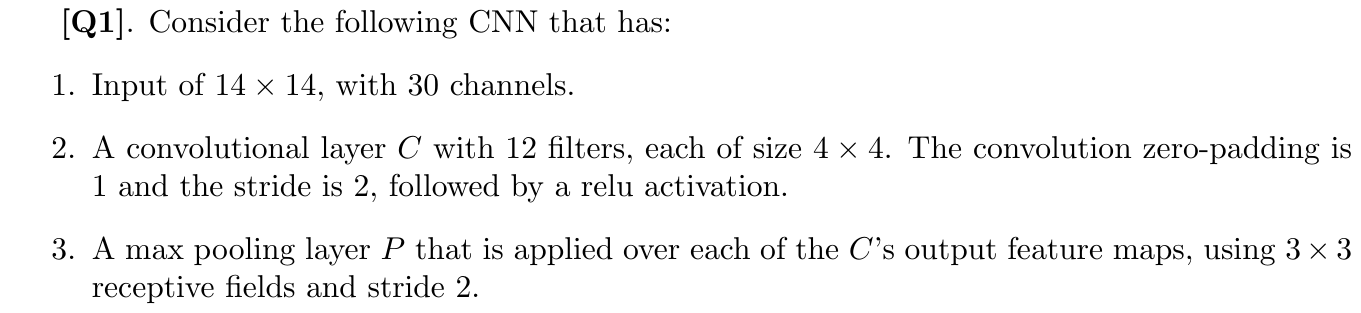
\includegraphics[width=\linewidth]{./assets/201806022206.png}
\end{figure}
\begin{enumerate}[label=\alph*)]
\item What is the total size of $C$'s output feature map?
\item What is the total size of $P$'s output feature map? 
\end{enumerate}
\begin{figure}[h!]
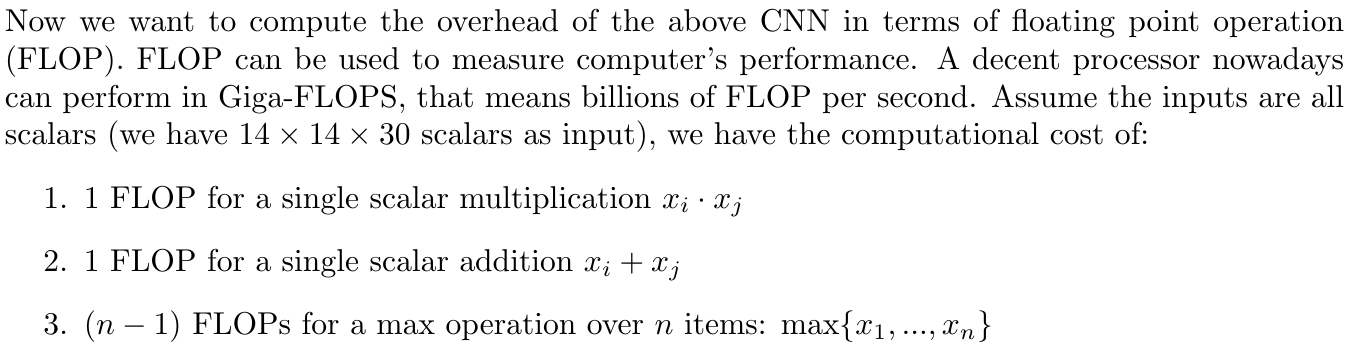
\includegraphics[width=\linewidth]{./assets/201806022208.png}
\end{figure}
\begin{enumerate}
\item[c)] How many FLOPs layer $C$ and $P$ cost in total to do one forward pass?
\end{enumerate}

\pagebreak

\begin{solution}{}~
\begin{enumerate}[label=\alph*)]
\item Output size: $O=\left\lfloor\frac{(W-K+2P)}{S}\right\rfloor+1$\\
$\begin{array}{rl}
O: & \text{Output size}\\
W: & \text{Input size}\\
K: & \text{Filter size}\\
P: & \text{Padding}\\
S: & \text{Stride}
\end{array}$\\

$\begin{aligned}
O&=\left\lfloor\frac{14-4+2}{2}\right\rfloor+1\\
&=7
\end{aligned}$\\

Size of $C$'s feature map: $7\times7\times12=588$
\item Output size: $O=\left\lfloor\frac{W-K}{S}\right\rfloor+1$\\
$\begin{array}{rl}
O: & \text{Output size}\\
W: & \text{Input size}\\
K: & \text{Filter size}\\
S: & \text{Stride}
\end{array}$\\

$\begin{aligned}
O&=\left\lfloor\frac{7-3}{2}\right\rfloor+1\\
&=3
\end{aligned}$\\

Size of $C$'s feature map: $3\times3\times12=108$
\item One convolution filter operation:\\
\begin{align*}
CF &= \text{Filter size}+(\text{Filter size}-1)\\
&= 16+15\\
&= 31
\end{align*}
One convolution operation:\\
\begin{align*}
C &= CF \times \text{Output size}\\
&= 31 \times 49\\
&= 1519
\end{align*}
One ReLU operation:\\
\begin{align*}
R &= \text{Input size}\\
&= 7\times7\\
&= 49
\end{align*}
One max pooling operation:\\
\begin{align*}
MP &= (\text{Filter size}-1)\times\text{Output size}\\
&= 8\times9\\
&= 72 
\end{align*}
Total FLOPs:\\
\begin{align*}
\text{Total} &= (C+R)\times\text{Number of filters}\times\text{Channels}+MP\times\text{Number of filters}\\
&= (1519+49)\times12\times30+72\times12\\
&= 565344
\end{align*}
\end{enumerate}
\end{solution}
\pagebreak
% Question 2
\begin{figure}[h!]
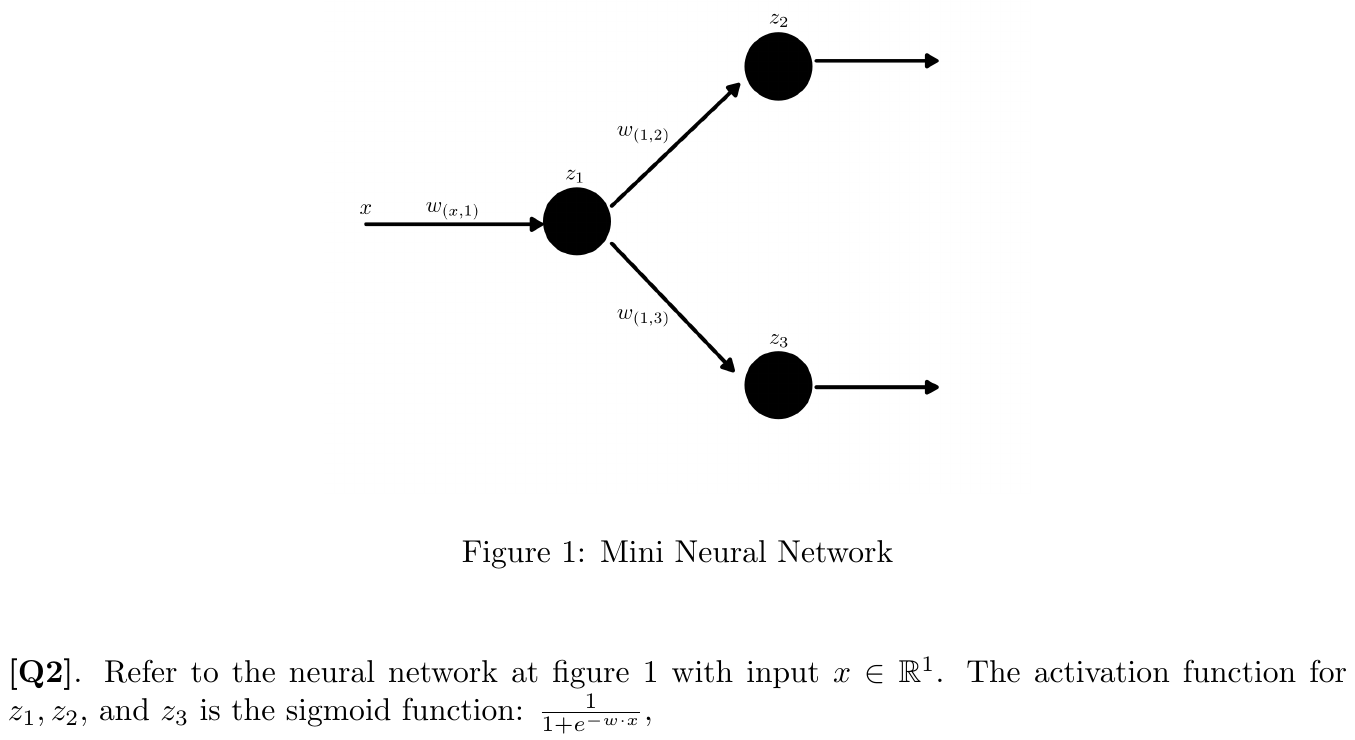
\includegraphics[width=\linewidth]{./assets/201806022242.png}
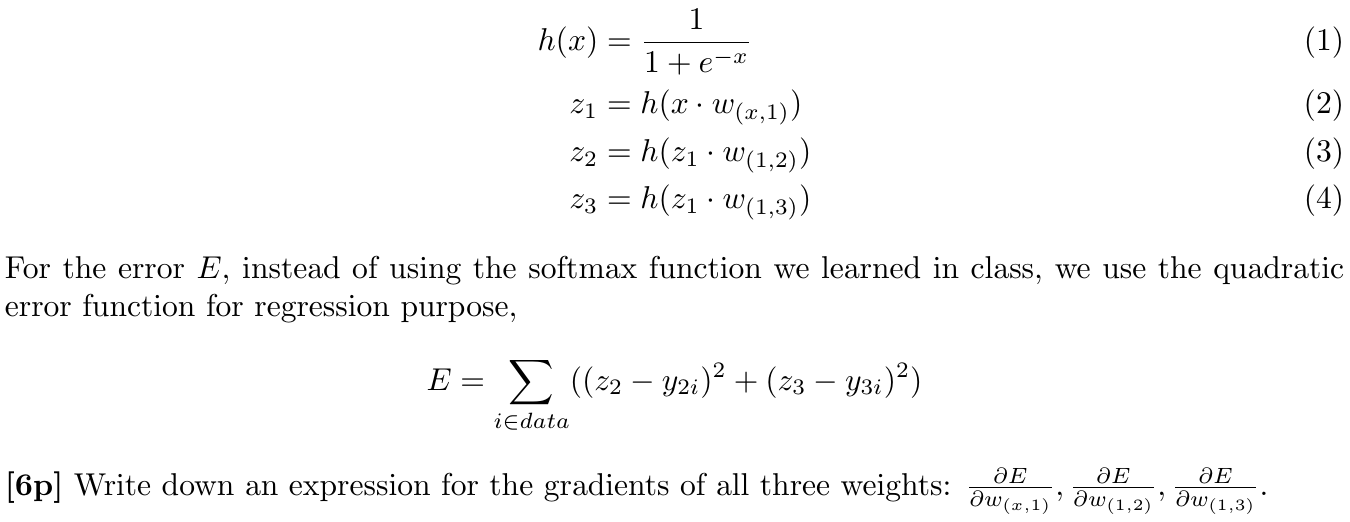
\includegraphics[width=\linewidth]{./assets/201806022243.png}
\end{figure}

\begin{solution}{}~
\begin{align*}
h(x)&=\frac{1}{1+e^{-x}}\\
h'(x)&=\frac{\delta h(x)}{\delta x}\\
&=\frac{e^{-x}}{(1+e^{-x})^2}\\
&=\frac{(1+e^{-x})-1}{(1+e^{-x})^2}\\
&=\frac{1}{1+e^{-x}}-\frac{1}{(1+e^{-x})^{2}}\\
&=h(x)-h(x)^2
\end{align*}
\begin{align*}
\frac{\delta z_1}{\delta w_{(x,1)}}&=xh'(x\cdot w_{(x,1)})\\
\text{The value of $z_1$ does not change}&\text{ with respect to }w_{(1,2)}\text{ and }w_{(1,3)},\\
\therefore\frac{\delta z_2}{\delta w_{(1,2)}}&=z_1h'(z_1\cdot w_{(1,2)})\\
\therefore\frac{\delta z_3}{\delta w_{(1,3)}}&=z_1h'(z_1\cdot w_{(1,3)})\\
\end{align*}
\begin{align*}
E &= \sum_{i\in data}((z_2-y_{2i})^2+(z_3-y_{3i})^2)\\
\frac{\delta E}{\delta z_2} &= \sum_{i\in data}2(z_2-y_{2i})\\
\frac{\delta E}{\delta z_3} &= \sum_{i\in data}2(z_3-y_{3i})\\
\frac{\delta z_2}{\delta z_1} &= w_{(1,2)}h'(z_1\cdot w_{(1,2)})\\
\frac{\delta z_3}{\delta z_1} &= w_{(1,3)}h'(z_1\cdot w_{(1,3)})
\end{align*}
\begin{align*}
\frac{\delta E}{\delta w_{(1,2)}} &= \frac{\delta E}{\delta z_2}\frac{\delta z_2}{\delta w_{(1,2)}}\\
&= z_1h'(z_1\cdot w_{(1,2)})\sum_{i\in data}2(z_2-y_{2i})\\
&= z_1(h(z_1\cdot w_{(1,2)})-h(z_1\cdot w_{(1,2)})^2)\sum_{i\in data}2(z_2-y_{2i})
\end{align*}
\begin{align*}
\frac{\delta E}{\delta w_{(1,3)}} &= \frac{\delta E}{\delta z_3}\frac{\delta z_3}{\delta w_{(1,3)}}\\
&= z_1h'(z_1\cdot w_{(1,3)})\sum_{i\in data}2(z_3-y_{3i})\\
&= z_1(h(z_1\cdot w_{(1,3)})-h(z_1\cdot w_{(1,3)})^2)\sum_{i\in data}2(z_3-y_{3i})
\end{align*}
\begin{align*}
\frac{\delta E}{\delta w_{(x,1)}} &= \frac{\delta E}{\delta z_2}\frac{\delta z_2}{\delta w_{(1,2)}}+\frac{\delta E}{\delta z_3}\frac{\delta z_3}{\delta w_{(1,3)}}\\
&= \frac{\delta E}{\delta z_2}\frac{\delta z_2}{\delta z_1}\frac{\delta z_1}{\delta w_{(x,1)}}+\frac{\delta E}{\delta z_3}\frac{\delta z_3}{\delta z_1}\frac{\delta z_1}{\delta w_{(x,1)}}\\
&= xw_{(1,2)}h'(z_1\cdot w_{(1,2)})h'(x\cdot w_{(x,1)})\sum_{i\in data}2(z_2-y_{2i})\\
&+ xw_{(1,3)}h'(z_1\cdot w_{(1,3)})h'(x\cdot w_{(x,1)})\sum_{i\in data}2(z_3-y_{3i})\\
&= xw_{(1,2)}(h(z_1\cdot w_{(1,2)})-h(z_1\cdot w_{(1,2)})^2)(h(x\cdot w_{(x,1)})-h(x\cdot w_{(x,1)})^2)\sum_{i\in data}2(z_2-y_{2i})\\
&+ xw_{(1,3)}(h(z_1\cdot w_{(1,3)})-h(z_1\cdot w_{(1,3)})^2)(h(x\cdot w_{(x,1)})-h(x\cdot w_{(x,1)})^2)\sum_{i\in data}2(z_3-y_{3i})
\end{align*}
\end{solution}

\section{Coding Component}

\lstinputlisting[language=Python]{pset3.py}

\end{document}
